\documentclass[10pt,twocolumn]{article}
\usepackage[margin=0.8in]{geometry}
\usepackage{amsmath,amssymb}
\usepackage{booktabs}
\usepackage{tikz}
\usepackage{graphicx}
\usepackage{hyperref}
\usepackage{microtype}

\title{Beating V8 \texttt{BigInt} Multiplication from WebAssembly}
\author{Julian Henry}
\date{September 2026}

\begin{document}
\maketitle

\begin{abstract}
A WebAssembly (WASM) multiplier beats V8's native \texttt{BigInt} multiply at every
operand size we tested from 16\,kbit to 33.5\,Mbit: $1.2$--$4.5\times$ faster in kernel
time and up to $2.9\times$ faster including conversion to and from \texttt{BigInt}.
The winning kernel is a SIMD double-precision FFT with balanced digits, a half-size
real-output inverse, and an $O(n)$ residue check with automatic retry. All 1,336 test
products matched V8 exactly, up to 1M limbs. A rebuilt in-place Karatsuba scales with
the textbook exponent but stays a constant $1.5\times$ behind V8's own Karatsuba,
because V8 multiplies 64-bit digits natively: no Karatsuba in WASM can overtake it; only
a lower-exponent algorithm can. We also show that the repository's previous Karatsuba
kernel returned wrong products for most random operands above 32 limbs.
\end{abstract}

\section{Background}
We measured V8's \texttt{a*b} (Node 26.5, V8 14.6, Apple M1 Pro). Up to about 2,048
32-bit limbs its time grows with local exponent $\approx 1.6$ (Karatsuba); beyond, the
exponent is $1.05$--$1.2$ (an FFT-class algorithm). V8 uses 64-bit digits with native
$64\times64\to128$-bit multiplies. WASM has none: this V8 rejects the
\texttt{wide-arithmetic} proposal's \texttt{i64.mul\_wide\_u}. A WASM kernel therefore
performs about $4\times$ more digit products at every size.

\paragraph{Why earlier attempts could not win.}
\begin{itemize}
\item \emph{Algorithm ceiling.} $O(n^{1.585})$ Karatsuba can at best tie V8's Karatsuba,
  and loses to V8's FFT above $\sim$2K limbs.
\item \emph{Allocation on the hot path.} The old \texttt{karatsuba.wat} bump-allocated and
  copied every split, sum and partial product; the old schoolbook allocated $\sim$3,000
  blocks ($\sim$16.7\,MB) per 1,024-limb multiply.
\item \emph{Benchmark artefacts.} The old harness timed an $O(n^2)$ \texttt{BigInt}-to-limbs
  conversion inside the WASM multiply, and reused the same operands every repetition.
  V8 hoists such loop-invariant \texttt{a*b}, and lowers \texttt{(a*b) \& 1n} to a 64-bit
  multiply; naive V8 timings read 3\,ns at every size.
\end{itemize}

\section{Methods}
All kernels are in \texttt{research/src/bigmul.c} (654 lines of C, a 21\,KB WASM module
with SIMD128). Numbers are little-endian 32-bit limbs; kernels write into caller-provided
buffers, so nothing is allocated during a multiply.

\paragraph{Karatsuba, rebuilt.} We use the subtractive form
\begin{equation}
a_0b_1 + a_1b_0 = a_0b_0 + a_1b_1 - (a_0-a_1)(b_0-b_1),
\end{equation}
so half-sums never grow a carry limb (the old kernel's bug class). Recursion uses one
$\sim4n$-limb scratch buffer. Below 96 limbs a SIMD Comba base case computes each column
as a contiguous dot product; \texttt{i64x2.extmul} forms two $32\times32$ products per
instruction, with low and high halves in separate 64-bit accumulators (no carry chain).

\paragraph{FFT multiply.} Five steps, all SIMD \texttt{f64x2} on split re/im arrays:
\begin{enumerate}
\item \textbf{Balanced digits.} Cut operands into $b$-bit digits in
  $[-2^{b-1}, 2^{b-1})$, with $b$ the largest value satisfying $2b + \log_2 N \le 56$
  ($b = 15$--$20$).
\item \textbf{One forward transform.} Pack $z = a + i\,b$; radix-4 DIF FFT of size $N$,
  depth-first until a sub-transform fits in L1 (4,096 points). Each radix-4 group loads one
  twiddle and derives the rest: $w(j+q) = -i\,w(j)$, $w_2 = w_1^2$.
\item \textbf{Pointwise product in scrambled order.}
  \begin{equation}
  A_kB_k = \frac{Z_k^2 - \overline{Z_{-k}}^{\,2}}{4i}.
  \end{equation}
  In bit-reversed order, the mirror of position $p \in [2^m, 2^{m+1})$ is
  $3\cdot2^m - 1 - p$, so no permutation pass is needed.
\item \textbf{Half-size inverse.} The product spectrum $C$ is Hermitian; fold it in place
  ($H = N/2$):
  \begin{equation}
  Z'_k = \bigl(C_k + \overline{C_{H-k}}\bigr) + i\,W^{-k}\bigl(C_k - \overline{C_{H-k}}\bigr),
  \end{equation}
  and $\mathrm{IFFT}_H(Z') = N(c_{2j} + i\,c_{2j+1})$. Transform work drops from $2N$ to $1.5N$.
\item \textbf{Round, carry, verify.} Accept only if the maximum rounding error is below
  $0.375$ and residues mod $2^{32}-1$ and $2^{31}-1$ match; otherwise retry with $b-1$.
  One wrong coefficient shifts the result by $\pm2^{bk} \not\equiv 0 \pmod{2^{32}-1}$, so it
  is always detected.
\end{enumerate}
\texttt{mul\_auto} uses Karatsuba below 216 limbs and the FFT above.

\begin{figure}[t]
\centering
% generated by make_figs.mjs
\resizebox{\columnwidth}{!}{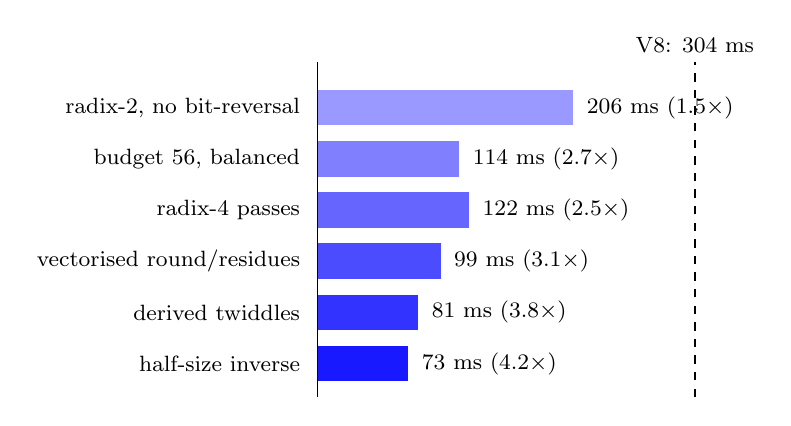
\begin{tikzpicture}[font=\footnotesize]
\fill[blue!40] (0,0.000) rectangle (3.246,0.450);
\node[anchor=east] at (-0.100,0.225) {radix-2, no bit-reversal};
\node[anchor=west] at (3.296,0.225) {206 ms (1.5$\times$)};
\fill[blue!50] (0,-0.650) rectangle (1.796,-0.200);
\node[anchor=east] at (-0.100,-0.425) {budget 56, balanced};
\node[anchor=west] at (1.846,-0.425) {114 ms (2.7$\times$)};
\fill[blue!60] (0,-1.300) rectangle (1.922,-0.850);
\node[anchor=east] at (-0.100,-1.075) {radix-4 passes};
\node[anchor=west] at (1.972,-1.075) {122 ms (2.5$\times$)};
\fill[blue!70] (0,-1.950) rectangle (1.560,-1.500);
\node[anchor=east] at (-0.100,-1.725) {vectorised round/residues};
\node[anchor=west] at (1.610,-1.725) {99 ms (3.1$\times$)};
\fill[blue!80] (0,-2.600) rectangle (1.276,-2.150);
\node[anchor=east] at (-0.100,-2.375) {derived twiddles};
\node[anchor=west] at (1.326,-2.375) {81 ms (3.8$\times$)};
\fill[blue!90] (0,-3.250) rectangle (1.150,-2.800);
\node[anchor=east] at (-0.100,-3.025) {half-size inverse};
\node[anchor=west] at (1.200,-3.025) {73 ms (4.2$\times$)};
\draw[black,thick,dashed] (4.790,-3.450) -- (4.790,0.8) node[above] {V8: 304 ms};
\draw (0,-3.450) -- (0,0.8);
\end{tikzpicture}}

\caption{Optimisation ladder at 1M limbs (33.5\,Mbit); each step measured after the
previous one. The dashed line is V8's time; ratios are speedups over V8.}
\label{fig:ladder}
\end{figure}

\section{Experimental setup}
Apple M1 Pro (arm64), Node 26.5.0 / V8 14.6.202.34; clang 24.0.0git
(\texttt{--target=wasm32 -O3 -msimd128}). Sizes 8 to 1,048,576 limbs (256\,bit to
33.5\,Mbit) at half-octave steps (35 sizes), balanced $n\times n$ products, seeded
xorshift128+ operands. Four distinct operand pairs rotate through 16 combinations; every
V8 product escapes to a global array; repetitions double until $\ge$60\,ms ($\ge$400\,ms
above 64K limbs); five interleaved trials, median reported (min--max spread $<2\%$ above
8 limbs). Kernel time assumes operands are in WASM memory; end-to-end time adds
\texttt{BigInt}$\to$hex$\to$limbs and back. Correctness: 1,336 exact comparisons against
V8 (all sizes 1--80 limbs; $2^p\pm1$, $2^p$, $1.37\cdot2^p$ for $p=7$--16; 262,144,
777,777 and 1,048,576 limbs; random and all-ones operands; six kernels).

\section{Results}
The WASM kernel beats V8 at every size from 16\,kbit (512 limbs) up:
$2.7$--$4.5\times$ at power-of-two sizes from 64\,kbit, $2.1$--$3.0\times$ just above them
(FFT padding). Below $\sim$12\,kbit V8 wins by $1.2$--$1.9\times$
(Fig.~\ref{fig:speedup}).

\begin{figure}[t]
\centering
% generated by make_figs.mjs
\resizebox{\columnwidth}{!}{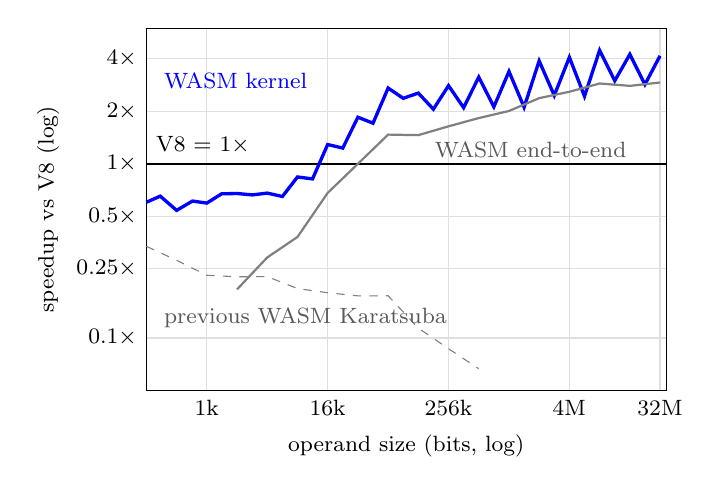
\begin{tikzpicture}[font=\footnotesize]
\draw[gray!25] (0,0.666) -- (6.6,0.666); \node[left] at (0,0.666) {$0.1\times$};
\draw[gray!25] (0,1.546) -- (6.6,1.546); \node[left] at (0,1.546) {$0.25\times$};
\draw[gray!25] (0,2.212) -- (6.6,2.212); \node[left] at (0,2.212) {$0.5\times$};
\draw[gray!25] (0,2.878) -- (6.6,2.878); \node[left] at (0,2.878) {$1\times$};
\draw[gray!25] (0,3.544) -- (6.6,3.544); \node[left] at (0,3.544) {$2\times$};
\draw[gray!25] (0,4.210) -- (6.6,4.210); \node[left] at (0,4.210) {$4\times$};
\draw[gray!25] (0.767,0) -- (0.767,4.6); \node[below] at (0.767,0) {1k};
\draw[gray!25] (2.302,0) -- (2.302,4.6); \node[below] at (2.302,0) {16k};
\draw[gray!25] (3.837,0) -- (3.837,4.6); \node[below] at (3.837,0) {256k};
\draw[gray!25] (5.372,0) -- (5.372,4.6); \node[below] at (5.372,0) {4M};
\draw[gray!25] (6.523,0) -- (6.523,4.6); \node[below] at (6.523,0) {32M};
\draw (0,0) rectangle (6.6,4.6);
\node at (3.3,-0.7) {operand size (bits, log)};
\node[rotate=90] at (-1.25,2.3) {speedup vs V8 (log)};
\draw[black,thick] (0,2.878) -- (6.6,2.878);
\node[anchor=south west] at (0.000,2.878) {V8 = $1\times$};
\draw[blue,very thick] plot coordinates {(0.000,2.390) (0.176,2.467) (0.384,2.287) (0.585,2.405) (0.767,2.379) (0.956,2.497) (1.151,2.501) (1.346,2.483) (1.535,2.506) (1.727,2.463) (1.919,2.711) (2.110,2.686) (2.302,3.123) (2.494,3.078) (2.686,3.470) (2.878,3.394) (3.070,3.840) (3.262,3.710) (3.453,3.776) (3.645,3.572) (3.837,3.871) (4.029,3.591) (4.221,3.979) (4.413,3.602) (4.605,4.051) (4.797,3.596) (4.988,4.185) (5.180,3.746) (5.372,4.231) (5.564,3.736) (5.756,4.320) (5.948,3.933) (6.140,4.269) (6.331,3.885) (6.523,4.249)};
\draw[gray,thick] plot coordinates {(1.151,1.283) (1.535,1.689) (1.919,1.949) (2.302,2.508) (2.686,2.878) (3.070,3.249) (3.453,3.242) (3.837,3.354) (4.221,3.459) (4.605,3.549) (4.988,3.712) (5.372,3.793) (5.756,3.898) (6.140,3.868) (6.523,3.911)};
\draw[gray,dashed] plot coordinates {(0.000,1.830) (0.384,1.653) (0.767,1.463) (1.151,1.443) (1.535,1.446) (1.919,1.293) (2.302,1.241) (2.686,1.201) (3.070,1.202) (3.453,0.792) (3.837,0.530) (4.221,0.276)};
\node[blue,anchor=west] at (0.101,3.934) {WASM kernel};
\node[gray!70!black,anchor=west] at (3.541,3.054) {WASM end-to-end};
\node[gray!70!black,anchor=west] at (0.101,0.918) {previous WASM Karatsuba};
\end{tikzpicture}}

\caption{Speedup over V8 \texttt{BigInt} (V8 time / WASM time). The zigzag is FFT
padding just above powers of two. WASM first wins at 16\,kbit and peaks at $4.5\times$
at 8\,Mbit. End-to-end includes the hex round trip.}
\label{fig:speedup}
\end{figure}

\paragraph{Scaling.} Fitted exponents (time $\propto$ size$^k$): over 4--64\,kbit, V8
$k=1.64$ and WASM Karatsuba $k=1.65$; over 128\,kbit--33\,Mbit, V8 $k=1.18$, WASM
Karatsuba $k=1.59$, WASM FFT $k=1.08$. Karatsuba runs parallel to V8; only the FFT bends
below it (Fig.~\ref{fig:scaling}). At 33.5\,Mbit Karatsuba is $98\times$ slower than the FFT.

\begin{figure}[t]
\centering
% generated by make_figs.mjs
\resizebox{\columnwidth}{!}{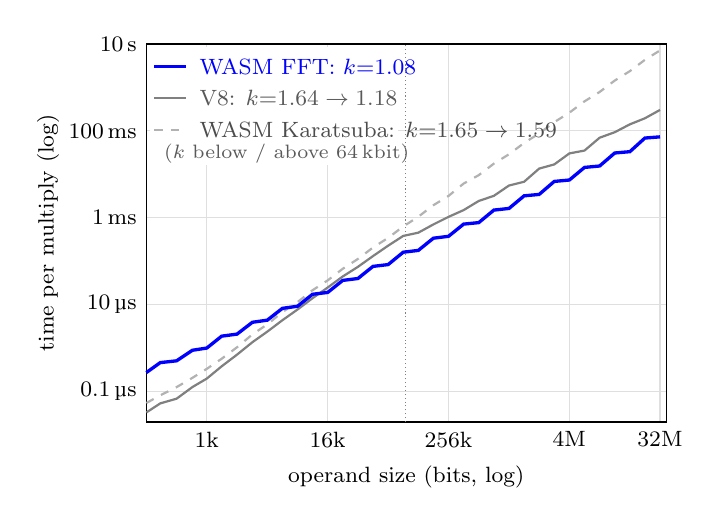
\begin{tikzpicture}[font=\footnotesize]
\draw[gray!25] (0,0.386) -- (6.6,0.386); \node[left] at (0,0.386) {0.1\,\textmu s};
\draw[gray!25] (0,1.490) -- (6.6,1.490); \node[left] at (0,1.490) {10\,\textmu s};
\draw[gray!25] (0,2.593) -- (6.6,2.593); \node[left] at (0,2.593) {1\,ms};
\draw[gray!25] (0,3.697) -- (6.6,3.697); \node[left] at (0,3.697) {100\,ms};
\draw[gray!25] (0,4.800) -- (6.6,4.800); \node[left] at (0,4.800) {10\,s};
\draw[gray!25] (0.767,0) -- (0.767,4.8); \node[below] at (0.767,0) {1k};
\draw[gray!25] (2.302,0) -- (2.302,4.8); \node[below] at (2.302,0) {16k};
\draw[gray!25] (3.837,0) -- (3.837,4.8); \node[below] at (3.837,0) {256k};
\draw[gray!25] (5.372,0) -- (5.372,4.8); \node[below] at (5.372,0) {4M};
\draw[gray!25] (6.523,0) -- (6.523,4.8); \node[below] at (6.523,0) {32M};
\draw (0,0) rectangle (6.6,4.8);
\node at (3.3,-0.7) {operand size (bits, log)};
\node[rotate=90] at (-1.25,2.4) {time per multiply (log)};
\draw[gray,densely dotted] (3.294,0) -- (3.294,4.8) node[below left,align=right,font=\scriptsize] {V8 switches\\to its FFT};
\draw[gray,thick] plot coordinates {(0.000,0.121) (0.176,0.236) (0.384,0.296) (0.585,0.444) (0.767,0.551) (0.956,0.707) (1.151,0.855) (1.346,1.013) (1.535,1.147) (1.727,1.292) (1.919,1.428) (2.110,1.572) (2.302,1.707) (2.494,1.848) (2.686,1.970) (2.878,2.107) (3.070,2.239) (3.262,2.363) (3.453,2.404) (3.645,2.509) (3.837,2.605) (4.029,2.691) (4.221,2.807) (4.413,2.872) (4.605,3.003) (4.797,3.051) (4.988,3.218) (5.180,3.271) (5.372,3.411) (5.564,3.447) (5.756,3.610) (5.948,3.680) (6.140,3.780) (6.331,3.857) (6.523,3.963)};
\draw[gray!60,thick,dashed] plot coordinates {(0.000,0.241) (0.176,0.338) (0.384,0.443) (0.585,0.561) (0.767,0.675) (0.956,0.803) (1.151,0.949) (1.346,1.112) (1.535,1.239) (1.727,1.396) (1.919,1.522) (2.110,1.673) (2.302,1.798) (2.494,1.946) (2.686,2.070) (2.878,2.216) (3.070,2.338) (3.262,2.483) (3.453,2.606) (3.645,2.753) (3.837,2.871) (4.029,3.028) (4.221,3.135) (4.413,3.281) (4.605,3.400) (4.797,3.544) (4.988,3.664) (5.180,3.808) (5.372,3.928) (5.564,4.072) (5.756,4.191) (5.948,4.336) (6.140,4.456) (6.331,4.599) (6.523,4.719)};
\draw[blue,very thick] plot coordinates {(0.000,0.628) (0.176,0.754) (0.384,0.777) (0.585,0.911) (0.767,0.939) (0.956,1.090) (1.151,1.116) (1.346,1.266) (1.535,1.293) (1.727,1.443) (1.919,1.470) (2.110,1.622) (2.302,1.645) (2.494,1.798) (2.686,1.822) (2.878,1.976) (3.070,1.999) (3.262,2.156) (3.453,2.179) (3.645,2.334) (3.837,2.358) (4.029,2.513) (4.221,2.532) (4.413,2.691) (4.605,2.712) (4.797,2.872) (4.988,2.890) (5.180,3.055) (5.372,3.073) (5.564,3.233) (5.756,3.251) (5.948,3.416) (6.140,3.433) (6.331,3.606) (6.523,3.621)};
\fill[white] (0.051,3.262) rectangle (3.201,4.762);
\draw[blue,very thick] (0.101,4.512) -- +(0.4,0);
\node[blue,anchor=west] at (0.551,4.512) {WASM FFT: $k{=}1.08$};
\draw[gray,thick] (0.101,4.112) -- +(0.4,0);
\node[gray!70!black,anchor=west] at (0.551,4.112) {V8: $k{=}1.64 \to 1.18$};
\draw[gray!60,thick,dashed] (0.101,3.712) -- +(0.4,0);
\node[gray!60!black,anchor=west] at (0.551,3.712) {WASM Karatsuba: $k{=}1.65 \to 1.59$};
\node[anchor=west,font=\scriptsize,gray!70!black] at (0.101,3.412) {($k$ below / above 64\,kbit)};
\end{tikzpicture}}

\caption{Time per $n\times n$ multiply (log--log) with fitted exponents
$k$ (time $\propto$ size$^k$). WASM Karatsuba stays parallel to V8's Karatsuba; only the
WASM FFT bends below V8's curve.}
\label{fig:scaling}
\end{figure}

\paragraph{Rounding error.} Unsigned digits average $2^{b-1}$, so their products add
coherently and error grows $\propto N$; balanced digits average zero and add like a
random walk. The gap grows with size: $53\times$ at 1K limbs, $\sim160\times$ at 16K,
$1{,}280\times$ at 1M (Fig.~\ref{tab:err}). At 1M limbs the policy picks 17 bits, with
worst observed error $0.014$.

\begin{figure}[t]
\centering
% generated by make_figs.mjs
\resizebox{\columnwidth}{!}{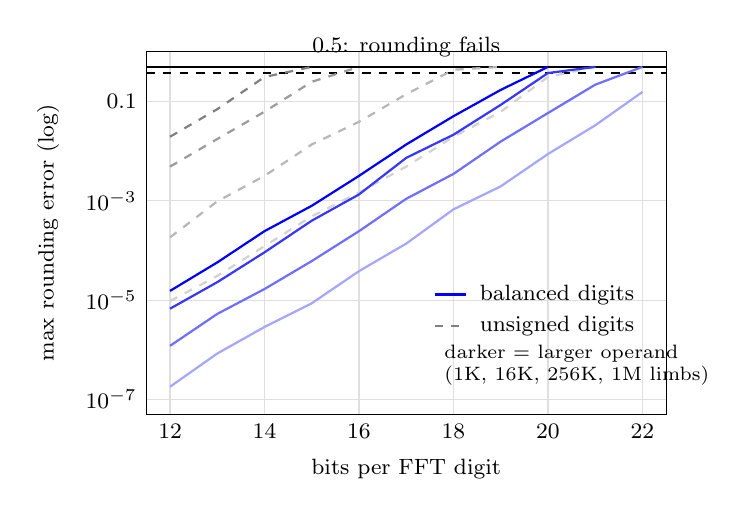
\begin{tikzpicture}[font=\footnotesize]
\draw[gray!25] (0,0.189) -- (6.6,0.189); \node[left] at (0,0.189) {$10^{-7}$};
\draw[gray!25] (0,1.449) -- (6.6,1.449); \node[left] at (0,1.449) {$10^{-5}$};
\draw[gray!25] (0,2.710) -- (6.6,2.710); \node[left] at (0,2.710) {$10^{-3}$};
\draw[gray!25] (0,3.970) -- (6.6,3.970); \node[left] at (0,3.970) {$0.1$};
\draw[gray!25] (0.300,0) -- (0.300,4.6); \node[below] at (0.300,0) {12};
\draw[gray!25] (1.500,0) -- (1.500,4.6); \node[below] at (1.500,0) {14};
\draw[gray!25] (2.700,0) -- (2.700,4.6); \node[below] at (2.700,0) {16};
\draw[gray!25] (3.900,0) -- (3.900,4.6); \node[below] at (3.900,0) {18};
\draw[gray!25] (5.100,0) -- (5.100,4.6); \node[below] at (5.100,0) {20};
\draw[gray!25] (6.300,0) -- (6.300,4.6); \node[below] at (6.300,0) {22};
\draw (0,0) rectangle (6.6,4.6);
\node at (3.3,-0.7) {bits per FFT digit};
\node[rotate=90] at (-1.25,2.3) {max rounding error (log)};
\draw[black,thick] (0,4.410) -- (6.6,4.410) node[pos=0.5,above] {0.5: rounding fails};
\draw[black,dashed] (0,4.332) -- (6.6,4.332);
\draw[blue!35,thick] plot coordinates {(0.300,0.348) (0.900,0.770) (1.500,1.107) (2.100,1.408) (2.700,1.816) (3.300,2.166) (3.900,2.601) (4.500,2.893) (5.100,3.304) (5.700,3.668) (6.300,4.092)};
\draw[gray!35,thick,dashed] plot coordinates {(0.300,1.436) (0.900,1.755) (1.500,2.134) (2.100,2.513) (2.700,2.814) (3.300,3.144) (3.900,3.523) (4.500,3.841) (5.100,4.282) (5.700,4.410)};
\draw[blue!56.66666666666667,thick] plot coordinates {(0.300,0.867) (0.900,1.273) (1.500,1.589) (2.100,1.944) (2.700,2.324) (3.300,2.735) (3.900,3.051) (4.500,3.462) (5.100,3.824) (5.700,4.184) (6.300,4.410)};
\draw[gray!56.66666666666667,thick,dashed] plot coordinates {(0.300,2.245) (0.900,2.703) (1.500,3.026) (2.100,3.425) (2.700,3.713) (3.300,4.063) (3.900,4.374) (4.500,4.410)};
\draw[blue!78.33333333333334,thick] plot coordinates {(0.300,1.339) (0.900,1.676) (1.500,2.055) (2.100,2.457) (2.700,2.790) (3.300,3.255) (3.900,3.549) (4.500,3.928) (5.100,4.332) (5.700,4.410)};
\draw[gray!78.33333333333334,thick,dashed] plot coordinates {(0.300,3.144) (0.900,3.494) (1.500,3.841) (2.100,4.221) (2.700,4.410)};
\draw[blue!100,thick] plot coordinates {(0.300,1.565) (0.900,1.927) (1.500,2.324) (2.100,2.646) (2.700,3.026) (3.300,3.425) (3.900,3.784) (4.500,4.118) (5.100,4.410)};
\draw[gray!100,thick,dashed] plot coordinates {(0.300,3.523) (0.900,3.873) (1.500,4.282) (2.100,4.410)};
\draw[blue,thick] (3.660,1.520) -- +(0.4,0);
\node[anchor=west] at (4.110,1.520) {balanced digits};
\draw[gray,thick,dashed] (3.660,1.120) -- +(0.4,0);
\node[anchor=west] at (4.110,1.120) {unsigned digits};
\node[anchor=west,font=\scriptsize,align=left] at (3.660,0.620) {darker = larger operand\\(1K, 16K, 256K, 1M limbs)};
\end{tikzpicture}}

\caption{Maximum FFT rounding error vs digit size for random operands of 1K, 16K, 256K
and 1M limbs (darker = larger). Balanced digits (solid) stay 50--1{,}280$\times$ below
unsigned digits (dashed); at 1M limbs the policy picks 17 bits (error $0.014$).}
\label{tab:err}
\end{figure}

\paragraph{Adversarial inputs.} Inputs whose balanced digits are all maximal and of one
sign reach error $0.5$ on the first attempt. The residue check caught every one; each
product was exact after one retry (1K--256K limbs) or two (1M limbs, 458\,ms).

\paragraph{End-to-end cost.} Converting \texttt{BigInt}s into WASM memory and back costs
about half as much as the multiply itself, so the end-to-end path breaks even with V8 at
32\,kbit and reaches $2.9\times$ at 33.5\,Mbit (Fig.~\ref{fig:e2e}).

\begin{figure}[t]
\centering
% generated by make_figs.mjs
\resizebox{\columnwidth}{!}{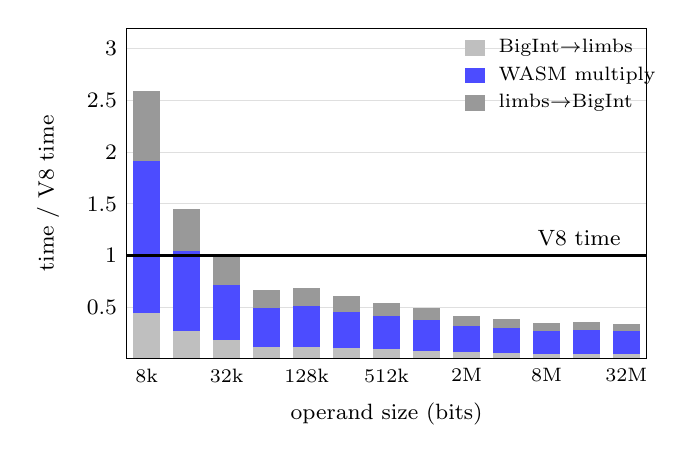
\begin{tikzpicture}[font=\footnotesize]
\draw[gray!25] (0,0.656) -- (6.6,0.656); \node[left] at (0,0.656) {0.5};
\draw[gray!25] (0,1.313) -- (6.6,1.313); \node[left] at (0,1.313) {1};
\draw[gray!25] (0,1.969) -- (6.6,1.969); \node[left] at (0,1.969) {1.5};
\draw[gray!25] (0,2.625) -- (6.6,2.625); \node[left] at (0,2.625) {2};
\draw[gray!25] (0,3.281) -- (6.6,3.281); \node[left] at (0,3.281) {2.5};
\draw[gray!25] (0,3.938) -- (6.6,3.938); \node[left] at (0,3.938) {3};
\fill[gray!50] (0.080,0.000) rectangle (0.428,0.584);
\fill[blue!70] (0.080,0.584) rectangle (0.428,2.513);
\fill[gray!80] (0.080,2.513) rectangle (0.428,3.405);
\node[below,font=\scriptsize] at (0.254,0.000) {8k};
\fill[gray!50] (0.588,0.000) rectangle (0.935,0.357);
\fill[blue!70] (0.588,0.357) rectangle (0.935,1.366);
\fill[gray!80] (0.588,1.366) rectangle (0.935,1.902);
\fill[gray!50] (1.095,0.000) rectangle (1.443,0.237);
\fill[blue!70] (1.095,0.237) rectangle (1.443,0.944);
\fill[gray!80] (1.095,0.944) rectangle (1.443,1.300);
\node[below,font=\scriptsize] at (1.269,0.000) {32k};
\fill[gray!50] (1.603,0.000) rectangle (1.951,0.157);
\fill[blue!70] (1.603,0.157) rectangle (1.951,0.649);
\fill[gray!80] (1.603,0.649) rectangle (1.951,0.879);
\fill[gray!50] (2.111,0.000) rectangle (2.458,0.155);
\fill[blue!70] (2.111,0.155) rectangle (2.458,0.668);
\fill[gray!80] (2.111,0.668) rectangle (2.458,0.895);
\node[below,font=\scriptsize] at (2.285,0.000) {128k};
\fill[gray!50] (2.618,0.000) rectangle (2.966,0.135);
\fill[blue!70] (2.618,0.135) rectangle (2.966,0.600);
\fill[gray!80] (2.618,0.600) rectangle (2.966,0.803);
\fill[gray!50] (3.126,0.000) rectangle (3.474,0.124);
\fill[blue!70] (3.126,0.124) rectangle (3.474,0.542);
\fill[gray!80] (3.126,0.542) rectangle (3.474,0.716);
\node[below,font=\scriptsize] at (3.300,0.000) {512k};
\fill[gray!50] (3.634,0.000) rectangle (3.982,0.107);
\fill[blue!70] (3.634,0.107) rectangle (3.982,0.494);
\fill[gray!80] (3.634,0.494) rectangle (3.982,0.647);
\fill[gray!50] (4.142,0.000) rectangle (4.489,0.087);
\fill[blue!70] (4.142,0.087) rectangle (4.489,0.420);
\fill[gray!80] (4.142,0.420) rectangle (4.489,0.543);
\node[below,font=\scriptsize] at (4.315,0.000) {2M};
\fill[gray!50] (4.649,0.000) rectangle (4.997,0.076);
\fill[blue!70] (4.649,0.076) rectangle (4.997,0.396);
\fill[gray!80] (4.649,0.396) rectangle (4.997,0.507);
\fill[gray!50] (5.157,0.000) rectangle (5.505,0.066);
\fill[blue!70] (5.157,0.066) rectangle (5.505,0.359);
\fill[gray!80] (5.157,0.359) rectangle (5.505,0.457);
\node[below,font=\scriptsize] at (5.331,0.000) {8M};
\fill[gray!50] (5.665,0.000) rectangle (6.012,0.064);
\fill[blue!70] (5.665,0.064) rectangle (6.012,0.371);
\fill[gray!80] (5.665,0.371) rectangle (6.012,0.468);
\fill[gray!50] (6.172,0.000) rectangle (6.520,0.063);
\fill[blue!70] (6.172,0.063) rectangle (6.520,0.356);
\fill[gray!80] (6.172,0.356) rectangle (6.520,0.448);
\node[below,font=\scriptsize] at (6.346,0.000) {32M};
\draw[black,thick] (0,1.313) -- (6.6,1.313) node[pos=0.97,above left] {V8 time};
\draw (0,0) rectangle (6.6,4.2);
\node at (3.3,-0.7) {operand size (bits)};
\node[rotate=90] at (-1.0,2.1) {time / V8 time};
\fill[gray!50] (4.3,3.85) rectangle +(0.25,0.2); \node[anchor=west,font=\scriptsize] at (4.6,3.95) {BigInt$\to$limbs};
\fill[blue!70] (4.3,3.5) rectangle +(0.25,0.2); \node[anchor=west,font=\scriptsize] at (4.6,3.6) {WASM multiply};
\fill[gray!80] (4.3,3.1500000000000004) rectangle +(0.25,0.2); \node[anchor=west,font=\scriptsize] at (4.6,3.25) {limbs$\to$BigInt};
\end{tikzpicture}}

\caption{End-to-end time split into conversion in, WASM multiply and conversion out,
relative to V8's \texttt{a*b} (bars below the line are faster than V8).}
\label{fig:e2e}
\end{figure}

\paragraph{Where FFT time goes.} The two transforms dominate: the forward transform takes
38--46\% and the half-size inverse about 16--21\%. The residue check costs 6--9\%
(Fig.~\ref{fig:profile}).

\begin{figure}[t]
\centering
% generated by make_figs.mjs
\resizebox{\columnwidth}{!}{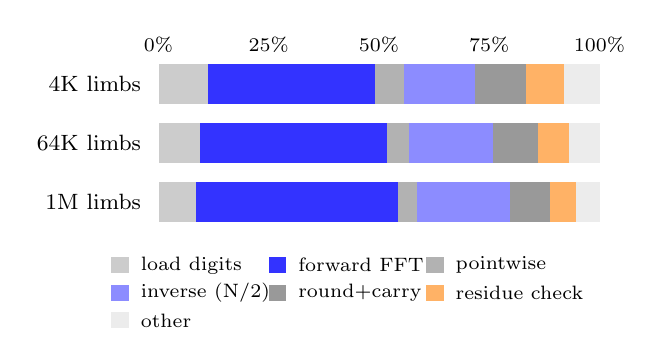
\begin{tikzpicture}[font=\footnotesize]
\fill[gray!40] (0.000,0) rectangle (0.622,0.5);
\fill[blue!80] (0.622,0) rectangle (2.752,0.5);
\fill[gray!60] (2.752,0) rectangle (3.111,0.5);
\fill[blue!45] (3.111,0) rectangle (4.021,0.5);
\fill[gray!80] (4.021,0) rectangle (4.667,0.5);
\fill[orange!60] (4.667,0) rectangle (5.145,0.5);
\fill[gray!15] (5.145,0) rectangle (5.6,0.5);
\node[anchor=east] at (-0.100,0.250) {4K limbs};
\fill[gray!40] (0.000,-0.75) rectangle (0.525,-0.25);
\fill[blue!80] (0.525,-0.75) rectangle (2.896,-0.25);
\fill[gray!60] (2.896,-0.75) rectangle (3.187,-0.25);
\fill[blue!45] (3.187,-0.75) rectangle (4.248,-0.25);
\fill[gray!80] (4.248,-0.75) rectangle (4.814,-0.25);
\fill[orange!60] (4.814,-0.75) rectangle (5.209,-0.25);
\fill[gray!15] (5.209,-0.75) rectangle (5.6,-0.25);
\node[anchor=east] at (-0.100,-0.500) {64K limbs};
\fill[gray!40] (0.000,-1.5) rectangle (0.474,-1);
\fill[blue!80] (0.474,-1.5) rectangle (3.046,-1);
\fill[gray!60] (3.046,-1.5) rectangle (3.283,-1);
\fill[blue!45] (3.283,-1.5) rectangle (4.460,-1);
\fill[gray!80] (4.460,-1.5) rectangle (4.974,-1);
\fill[orange!60] (4.974,-1.5) rectangle (5.298,-1);
\fill[gray!15] (5.298,-1.5) rectangle (5.6,-1);
\node[anchor=east] at (-0.100,-1.250) {1M limbs};
\fill[gray!40] (-0.6,-2.15) rectangle +(0.22,0.2); \node[anchor=west,font=\scriptsize] at (-0.35,-2.05) {load digits};
\fill[blue!80] (1.4,-2.15) rectangle +(0.22,0.2); \node[anchor=west,font=\scriptsize] at (1.65,-2.05) {forward FFT};
\fill[gray!60] (3.4,-2.15) rectangle +(0.22,0.2); \node[anchor=west,font=\scriptsize] at (3.65,-2.05) {pointwise};
\fill[blue!45] (-0.6,-2.5) rectangle +(0.22,0.2); \node[anchor=west,font=\scriptsize] at (-0.35,-2.4) {inverse (N/2)};
\fill[gray!80] (1.4,-2.5) rectangle +(0.22,0.2); \node[anchor=west,font=\scriptsize] at (1.65,-2.4) {round+carry};
\fill[orange!60] (3.4,-2.5) rectangle +(0.22,0.2); \node[anchor=west,font=\scriptsize] at (3.65,-2.4) {residue check};
\fill[gray!15] (-0.6,-2.8499999999999996) rectangle +(0.22,0.2); \node[anchor=west,font=\scriptsize] at (-0.35,-2.7499999999999996) {other};
\foreach \p in {0,25,50,75,100} {\node[font=\scriptsize] at (5.6*\p/100,0.75) {\p\%};}
\end{tikzpicture}}

\caption{Share of FFT-multiply time per pipeline stage, measured stage by stage.
``Other'' is the Hermitian fold and call overhead.}
\label{fig:profile}
\end{figure}

\section{Discussion}
\paragraph{Is beating V8 impossible?} Not in general, only within the same algorithm
class. In the Karatsuba regime both implementations share the exponent, so the
$1.47$--$1.52\times$ constant gap from V8's 64-bit digits never closes. Above 2,048 limbs
V8 switches to its FFT ($k=1.18$) and WASM Karatsuba falls $23\times$ behind at 1M
limbs. Overtaking requires an FFT with better constants than V8's own; ours scales at
$k=1.08$.

\paragraph{The previous kernel was wrong.} \texttt{karatsuba.wat} stores
$x_\text{low}+x_\text{high}$ in an $(m{+}1)$-limb block but copies only $m$ limbs; a
carry then adds stale heap contents. It passes on zeroed memory (how the old tests ran).
With a reused heap, random operands failed at 48 limbs in 17/20 trials and at every size
$\ge96$ limbs in 20/20; its own recursion reuses memory, so it fails within one call at
depth $\ge2$. One \texttt{i32.store} of zero fixes it. Fixed, it is $3.8\times$ slower
than the new Karatsuba and $10.6\times$ slower than the FFT at 1,024 limbs.

\paragraph{Limitations.} One machine and engine; balanced $n\times n$ only; a padding
sawtooth; exactness rests on verification, not proof; adversarial inputs cost retries
($1.5\times$ slower than V8 at 1M limbs); end-to-end pays only from $\sim$1,024 limbs;
FFT memory $\approx5N$ doubles ($\sim$170\,MB at 1M limbs), capping operands near 20M
limbs under wasm32.

\paragraph{Future work.} \texttt{wide-arithmetic} for 64-bit digits; mixed-radix or
truncated FFTs; Toom-3 for 128--400 limbs; worker threads; an NTT for proof-level
exactness.

\end{document}
